\section*{A: Ping Sweeping}
Ping sweep using angry IP of my home network.\\
\begin{figure}[H]
    \centering
    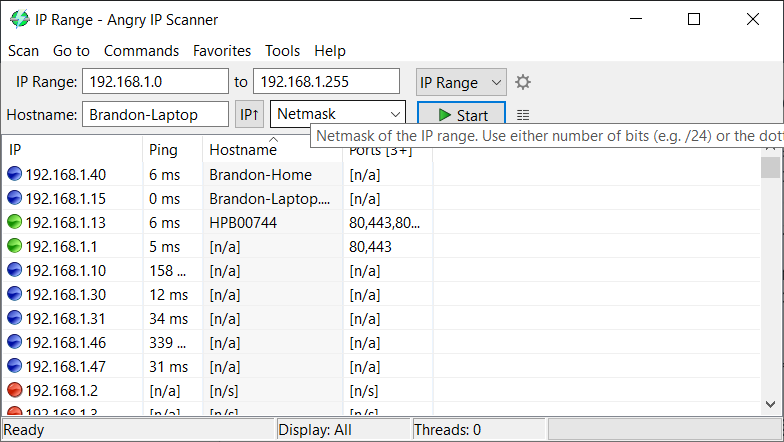
\includegraphics[width=\linewidth]{figures/a1.png}
    \caption{Angry IP output.}
\end{figure}
The output of Angry IP shows that the devices connected to the network that respond to pings and if some specified ports are opened.

\section*{B: Port Scanning}
Using the Zenmap tool I scanned Florida Poly's IP address using \verb|SYN| scan, \verb|NULL| scan, \verb|XMAS| scan and a Connection scan.

\begin{figure}[H]
    \centering
    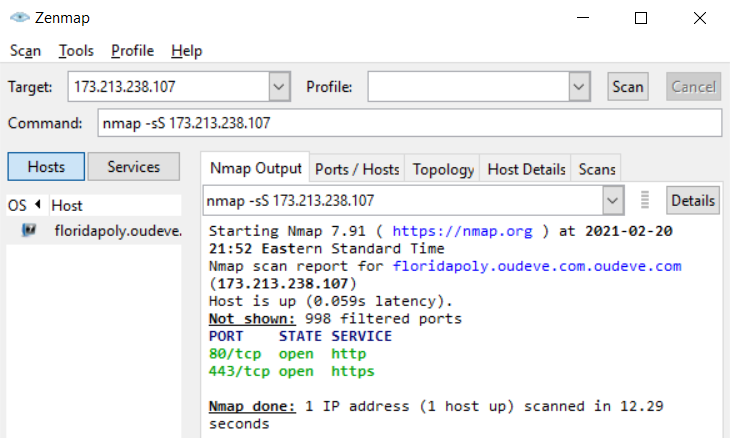
\includegraphics[width=\linewidth]{figures/b1.png}
    \caption{Zenmap output of SYN scan.}
\end{figure}
Half connect scan shows open ports via TCP but does not send the final ACK packet.
This scan tends to be faster and is less likely to be logged than the full connection scan.

\begin{figure}[H]
    \centering
    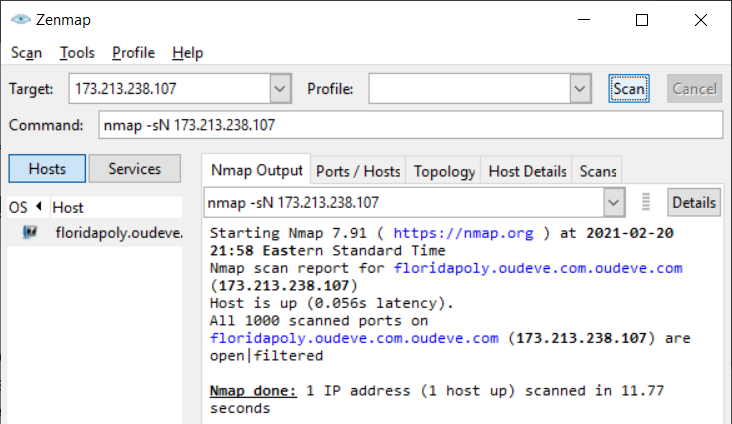
\includegraphics[width=\linewidth]{figures/b2.png}
    \caption{Zenmap output of NULL scan.}
\end{figure}
This scan sends packets with no flags enabled.
Very clearly defines if ports are opened or closed.

\begin{figure}[H]
    \centering
    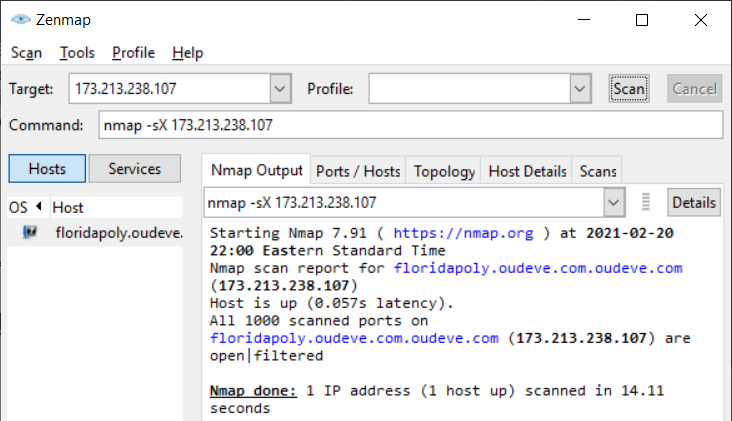
\includegraphics[width=\linewidth]{figures/b3.png}
    \caption{Zenmap output of XMAS scan.}
\end{figure}
This scan sends packets with multiple flags enabled.
If there is no response from the target it typically means that the port is open.

\begin{figure}[H]
    \centering
    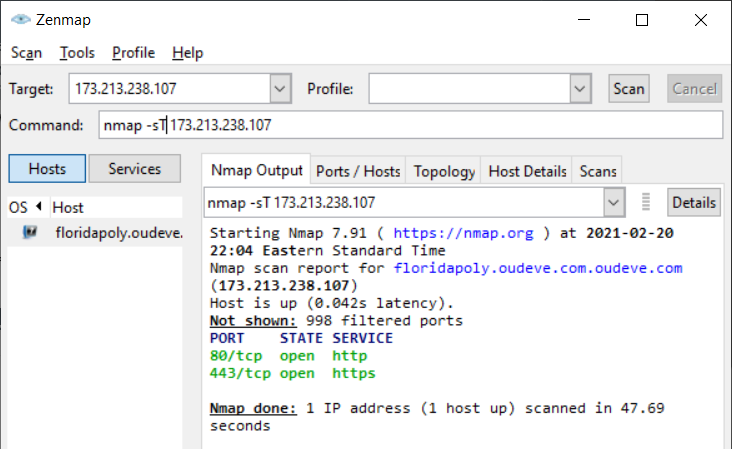
\includegraphics[width=\linewidth]{figures/b4.png}
    \caption{Zenmap output of full connect scan}
\end{figure}
The Full connect scan identifies open ports via a completed TCP handshake.
This scan is more likely to be logged.

\section*{C: Packet Crafting}
Kali Linux's \verb|hping3| tool is used to craft a packet and receive a response from the target.

\begin{figure}[H]
    \centering
    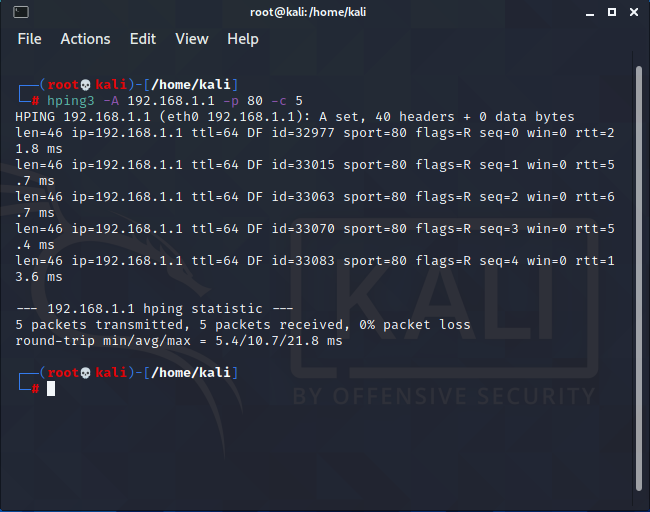
\includegraphics[width=\linewidth]{figures/c1.png}
    \caption{Hping3 with ACK scan on port 80.}
\end{figure}

In this lab we used network scanning tools to show devices on the network, ports that are open on devices and crafting packets.
This is the process of scanning a network to discover the structure of the network and connected hosts.
The Angry IP scan shows devices on the network that are available and online.
Zenmap scans a specific IP for open ports using a variety of different scanning types meant to trick the system into giving a response despite a firewall or other countermeasure.
Lastly, Kali Linux's Hping3 tool crafts a packet to send to an IP with the ability to specify flags.